\chapter{Grundlagen}
\label{chap:basics}

Bevor die Ziele der Migration von Flow zu TypeScript im nächsten Kapitel dargelegt werden, sollen zunächst die nötigen theoretischen Grundlagen erörtert werden, um die Nachvollziehbarkeit der weiteren Ausführungen zu erleichtern.

\section{Konzepte und Begriffe der Typentheorie}

\subsection{Korrektheit von Typsystemen}
Ein wichtiges Konzept aus der Theorie der Typensysteme ist deren logische \textit{Korrektheit} (engl. \textit{soundness}). Dieses Kriterium beschreibt, ob das System garantieren kann, dass ein Programm während dessen Ausführung tatsächlich keine Typfehler verursacht, sofern keine statischen Typverletzungen bestehen~\autocite{WRIGHT:1994}. In einem solchen Typsystem stimmt also der Typ eines zur Laufzeit ausgewerteten Ausdrucks immer mit dem statischen Typ überein~\autocite{DART:TYPE_SYSTEM}. Durch mathematische Formalisierung des Systems kann diese Eigenschaft bewiesen werden~\autocite[7]{CARDELLI:TYPE_SYSTEMS}. Das Gegenstück von Korrektheit ist \textit{Vollständigkeit}. Während ein korrektes System alle Fehler identifiziert, die zur Laufzeit auftreten können, findet ein vollständiges System nur diejenigen Fehler, die tatsächlich eintreten würden~\autocite{FLOW:TYPES_AND_EXPRESSIONS}. Im ersten Fall werden unter Umständen Fehler entdeckt, die zur Laufzeit praktisch nicht vorkommen (falsch positiver Fehler), im zweiten Fall treten dagegen eventuell Laufzeitfehler auf, obwohl keine Typverletzung festgestellt wurde (falsch negativer Fehler). Im Idealfall ist ein Typsystem sowohl korrekt, als auch vollständig.

Das Typsystem mancher Programmiersprachen erfüllt diese Definition von Korrektheit nicht. Im Fall von C ist die Semantik bestimmter Operationen wie beispielsweise die Dereferenzierung des Nullzeigers in der Sprachspezikation undefiniert~\autocite[79]{ISO:C99}. Obwohl ein solches Programm durch den Compiler akzeptiert wird, also keine Typverletzungen aufweist, können so Laufzeitfehler auftreten.

\subsection{Nominale und strukturelle Typen}
Eine Möglichkeit Typsysteme zu klassifizieren ist die Verwendung von \textit{nominalen} bzw. \textit{strukturellen} Typen. Relevant ist dabei die Fragestellung, ob unabhängige Typen durch das Typsystem als äquivalent angesehen werden oder nicht~\autocite[9]{CARDELLI:TYPE_SYSTEMS}. Bedeutsam ist auch, wann ein Typ als Untertyp eines anderen Typen betrachtet wird. Bei strukturellen Typen liegt ein Subtyp vor, wenn dessen Attribute eine Obermenge des Supertyps sind~\autocite{MALAYERI:2008}. Liegt hingegen ein nominaler Typ vor, so besteht eine solche Beziehung nur genau dann , wenn sie explizit deklariert wird (zum Beispiel durch das Schlüsselwort \code{extends}). Die Typsysteme der meisten realen Programmiersprachen setzen sowohl nominale, als auch strukturelle Typen ein~\autocite[9]{CARDELLI:TYPE_SYSTEMS}. Anhand eines Beispiels in Pseudocode (Quelltext~\ref{code:type-equivalence}) soll diese Differenzierung verdeutlicht werden.

\begin{lstlisting}[
  label={code:type-equivalence},
  caption={Beispiel zur Differenzierung von nominalen und strukturellen Typen.}
]
class A { prop: string; }
class B { prop: string; }
function f(arg: A) {}
f(new B()); // << Typfehler?
\end{lstlisting}

In den ersten beiden Zeilen werden zunächst zwei Klassen \code{A} und \code{B} definiert. Weiterhin wird eine Funktion \code{f} angegeben, die einen Parameter vom Typ \code{A} erwartet. Bei Aufruf dieser Funktion mit einer Instanz der Klasse \code{B} sind nun zwei Fälle möglich: Entweder spezifiziert das System, dass Typen mit unterschiedlichen Namen stets inkompatibel sind oder die Typen \code{A} und \code{B} werden als äquivalent betrachtet, da ihre Struktur übereinstimmt. Im ersten Fall würde in Zeile 4 eine Typverletzung auftreten, da der Typ des Ausdrucks \code{new B()} nicht \code{A}, sondern \code{B} ist. Läge hingegen eine strukturelle Typisierung vor, so würde das Programm akzeptiert werden, da der Aufbau der Klassen \code{A} und \code{B} identisch ist. Beide enthalten genau ein Attribut \code{prop} mit demselben Typ \code{string}.

\section{Statische Typsysteme für JavaScript}
\label{sec:static-typesystems-for-js}

Im Folgenden sollen bestehende statische Typsysteme für JavaScript betrachtet werden. Die Idee die ausgeführten Schwachstellen der dynamischen Typisierung der Sprache durch statische Systeme auszugleichen ist nicht neu~\autocite[2]{FLOW:PAPER}. Innerhalb der letzten Jahre sind verschiedene Ansätze entstanden, die sich dieser Problematik widmen.

Ein Beispiel ist das 2009 erschienene Werkzeug \textit{Closure Compiler}~\autocite{CLOSURE:COMPILER}. Ziel dieses Transpilers ist es einerseits gängige Programmierfehler in JavaScript-Quelltexten mittels statischer Analyse aufzudecken, andererseits effizienteren Ausgabecode durch Anwendung verschiedener Optimierungen zu erzeugen~\autocite{CLOSURE:COMPILER}. Dabei ist es auch möglich Ausdrücke innerhalb des Quelltexts durch spezielle Annotationen in Kommentarblöcken zu typisieren, sodass der Compiler daraufhin die Typkorrektheit statisch überprüfen kann~\autocite{CLOSURE:TYPES}.

Einen anderen Ansatz verfolgt die Programmiersprache \textit{Dart}~\autocite{DART:SPEC}. Dart bietet ein gemäß obiger Definition korrektes, statisches Typsystem, welches neben konventionellen Typdeklarationen auch Typinferenz unterstützt~\autocite{DART:TYPE_SYSTEM}. Anstatt JavaScript-Code durch Typannotationen in Kommentaren zu erweitern, wird hier also auf eine andere Programmiersprache zurückgegriffen, um statische Typüberprüfungen zu erzielen. Um ein Dart-Programm in standardkonformes JavaScript zu übersetzen, kann der Transcompiler \textit{dart2js}~\autocite{DART:DART2JS} verwendet werden. In den nachfolgenden Abschnitten sollen nun die zwei in dieser Arbeit behandelten Systeme \textit{Flow}~\autocite{FLOW:PAPER} und \textit{TypeScript}~\autocite{TYPESCRIPT:SPEC} näher beleuchtet werden.

\subsection{Flow}
\label{subsec:flow}

\subsubsection{Charakterisierung}

Flow~\autocite{FLOW:PAPER} ist ein durch das US-amerikanische Unternehmen \textit{Facebook Inc.} entwickeltes Software"=System, das statische Typüberprüfungen in JavaScript durch das Einfügen von Typannotationen ermöglicht (s. Quelltext~\ref{code:example-flow}). Die Annotationen sind syntaktische Spracherweiterungen und müssen vor Auslieferung des Codes mittels eines geeigneten Werkzeugs wie beispielsweise Babel~\autocite{BABEL} entfernt werden, damit wieder regulärer JavaScript-Quelltext entsteht~\autocite{FLOW:INSTALLATION}.
Der Entwurf und die Implementierung von Flow wird in der akademischen Arbeit \enquote{\textit{Fast and Precise Type Checking for JavaScript}} von \citeauthor{FLOW:PAPER} ausführlich beschrieben. Die nachfolgenden Erläuterungen beziehen sich vorrangig auf den Inhalt dieser Veröffentlichung.

% TODO: Sind die Belege hier überall nötig..?
Flow verfolgt zwei primäre Ziele~\autocite{FLOW:TYPE_SYSTEM}: Erstens soll eine möglichst hohe Präzision durch die Typüberprüfungen erreicht werden, um möglichst zuverlässige Ergebnisse, das heißt eine geringe Quote falsch positiver und falsch negativer Fehler, zu erzielen. Zweitens müssen diese Ergebnisse selbst bei einer sehr umfangreichen Codebasis schnell berechnet werden können, damit der Workflow des Programmierers nicht verlangsamt wird.
Die erste Zielvorgabe wird zum einen anhand einer pfadsensitive Datenflussanalyse, zum anderen durch die Korrektheit des Typsystems realisiert~\autocite{FLOW:TYPE_SYSTEM}. Mittels pfadsensitiver Datenflussanalyse kann das Laufzeitverhalten von Software modelliert und so der Typ von Ausdrücken durch Einbeziehung der Programmverzweigungen auf einen spezielleren Untertyp abgebildet werden (\textit{type refinement})~\cites{WINTER:2013}[2]{FLOW:PAPER}. Um die Korrektheit des Typsystems zu gewährleisten, überprüft Flow \emph{alle} möglichen Werte innerhalb eines Ausdrucks~\autocite{FLOW:TYPES_AND_EXPRESSIONS}. Wie ausgeführt birgt dies die Gefahr Typfehler zu erkennen, die zur Laufzeit gar nicht auftreten würden.
Um das zweite Ziel, die Geschwindigkeit der Typüberprüfungen, zu steigern, wird das Verfahren modularisiert, sodass die Berechnungen stark parallelisiert werden können~\autocite[4]{FLOW:PAPER}. Flow nutzt hierbei aus, dass in modernen JavaScript-Projekten üblicherweise genau eine Datei pro Modul vorliegt. Unabhängige Module können somit durch mehrere unabhängige Prozesse auf verschiedenen Rechenkernen gleichzeitig überprüft werden. Die Ergebnisse dieser Berechnungen werden daraufhin durch einen MapReduce-Algorithmus, der auf einer geteilten Heap-Datenstruktur arbeitet, rekombiniert~\autocite[22\psq]{FLOW:PAPER}.

Die Architektur von Flow gliedert sich in einen Server, einen Client und einen Dateisystemüberwacher~\autocite[22]{FLOW:PAPER}. Der Server liest zunächst den Quelltext des gesamten Projekts ein und überprüft diesen hinsichtlich Typverletzungen. Daraufhin läuft der Prozess im Hintergrund weiter und ist bereit Anfragen des Clients entgegen zu nehmen. Der Client -- zum Beispiel die integrierte Entwicklungsumgebung -- kann nun durch Kommandos einerseits den generellen Status der Typüberprüfung abrufen, andererseits spezifischere Informationen wie beispielsweise den Typ eines bestimmten Ausdrucks abfragen. Sobald eine Datei editiert, neu erstellt oder gelöscht wird, wird dies dem Server durch den Dateisystemüberwacher mitgeteilt. Daraufhin überprüft der Server die Typkorrektheit inkrementell erneut auf Grundlage des modifizierten Quelltexts. Dabei werden nur geänderte Module und deren Abhängigkeiten betrachtet, sodass der Berechnungs- und damit Zeitaufwand stark reduziert werden kann. Weil die aktuellen Ergebnisse stets im Arbeitsspeicher vorgehalten werden, können nachfolgende Anfragen des Clients schnell beantwortet werden.

Flow ist in der Lage Typen global zu inferieren~\autocite[25]{FLOW:PAPER}. Das heißt der Typ vieler Ausdrücke muss nicht explizit angegeben werden, sondern kann durch das Typsystem selbstständig abgeleitet werden. Deshalb kann bereits mit wenigen expliziten Annotationen eine hohe Abdeckung der Codebasis durch das Typsystem erzielt werden~\autocite[24]{FLOW:PAPER}. Eine weitere Eigenschaft des Typsystems ist die Verwendung von nominalen und strukturellen Typen. Flow behandelt Klassen und opake Typen (s. Tabelle~\ref{tab:flow-base-types}) nominal, alle anderen Typen hingegen strukturell~\autocite{FLOW:NOMINAL_TYPES}.

\subsubsection{Beispiel}

Zur Veranschaulichung wie Flow benutzt wird, soll in Quelltext~\ref{code:example-flow} die Typisierung eines einfachen JavaScript-Programms anhand des Algorithmus der linearen Suche demonstriert werden. In diesem und allen weiteren Quelltexten werden dabei die Schlüsselworte von JavaScript bzw. TypeScript \code{\textbf{fett}} und Typannotationen \code{\textit{kursiv}} abgedruckt.

\begin{lstlisting}[
  label={code:example-flow},
  caption={Benutzung von Flow anhand des Algorithmus der linearen Suche.},
  mathescape=true,
]
// @flow
function linearSearch<T>(list: Array<T>, searchValue: T): number | empty {
  for (const [index, value] of list.entries()) {
    if (value === searchValue) {
      return index;
    }
  }
  throw new Error('Not found');
}

linearSearch<number>([3, 1, 10, 56], 10);        // $\rightarrow$ 2
linearSearch<number>([3, 1, 10, 56], 12);        // $\rightarrow$ Exception (Not Found)
linearSearch<string>(['foo', 'bar', 'baz'], 3);  // $\rightarrow$ Typfehler (3 ist kein String)
\end{lstlisting}

Im Beispiel werden verschiedene Sprachkonstrukte von Flow eingesetzt: Zunächst wird in Zeile 4 die Funktion \code{linearSearch} definiert, die den Suchalgorithmus implementiert. Deren formale Parameter werden dabei durch einen generischen Typparameter \code{T} typisiert. Hierdurch wird festgelegt, dass das erste Argument ein homogenes Feld mit Werten dieses Typs \code{T} und der zweite Parameter \code{searchValue} ein Wert desselben Typs sein muss. Mittels dieser Einschränkung werden unsinnige Funktionsaufrufe mit Suchwerten, die aufgrund der Typisierung gar nicht Bestandteil des Felds sein \emph{können}, statisch erkannt (vgl. Zeile 13). Der Algorithmus liefert entweder den Feldindex des Suchwerts zurück, sofern dieser in der Liste vorkommt, oder löst eine \textit{Exception} aus\footnote{Das Auslösen einer Exception an dieser Stelle ist aus softwaretechnischer Perspektive fragwürdig, verbessert aber die Ausdruckskraft des Beispiels.}. Flow bietet für den zweiten Fall den adäquaten Typ \code{empty}, welcher dem leeren Typ (\textit{bottom type} $\bot$) entspricht. Der korrekte Rückgabetyp der Funktion ist somit die Vereinigung aus \code{number} und \code{empty} (\textit{Union type}). Der Typ aller Ausdrücke im Funktionskörper kann durch Flow inferiert werden.

Nachfolgend sollen nun die verschiedenen Typen von Flow kurz beschrieben werden. Diese lassen sich in drei Kategorien einordnen: Basistypen, Hilfstypen und Typdeklarationen.
Unter Basistypen werden in dieser Arbeit die regulären Typannotationen von Flow verstanden. Diese machen den größten Teil der Online-Dokumentation~\autocite{FLOW:TYPE_ANNOTATIONS} aus.
Hilfstypen (\textit{Utility types}) sind spezielle Typen, die einen oder mehrere andere Typen als Argument erhalten und so einen neuen Typ mit zusätzlichen, nützlichen Eigenschaften herstellen.
Typdeklarationen ermöglicht es schließlich die Schnittstellen externer Bibliotheken und Frameworks durch spezielle Deklarationsdateien zu typisieren. Auf diese Weise kann auch die Benutzung dieser Abhängigkeiten statisch überprüft werden.

\subsubsection{Basistypen}
\label{subsec:flow:base-types}

Tabelle~\ref{tab:flow-base-types} listet die Basistypen von Flow auf, beschreibt deren Zweck und zeigt ein Beispiel. Um die Nachvollziehbarkeit zur Online"=Dokumentation und der in Kapitel~\ref{chap:implementation} ausgeführten Implementierung zu erleichtern, werden die englischen Typbezeichnungen beibehalten und nicht ins Deutsche übersetzt.

\bigbreak
\begin{longtabuenv}
\begin{longtabu} to \textwidth {@{}>{\raggedright}p{2.75cm}CX[l]@{}}
    \midrule
    \libertineSB{Basistyp} & \libertineSB{Beispiel} & \libertineSB{Kurzbeschreibung} \\
    \midrule
  \endhead
    \midrule
    \caption{Basistypen von Flow~\autocite{FLOW:TYPE_ANNOTATIONS} mit Beispiel.}
  \endfoot
  Any type                 & any                             & Typ für beliebige Werte. Jeder Typ ist Subtyp von \code{any}. \code{any} ist jedem Typ zuweisbar und jeder Typ ist \code{any} zuweisbar. \medskip\\
  Array type               & Array<number>                   & Felder. Der Typparameter (hier \code{number}) gibt den Typ der Feldelemente an. \medskip\\
  Array type (shorthand)   & number[]                        & Felder (Kurzschreibweise). \medskip\\
  Boolean literal type     & true                            & Boolesche Literale (entweder \code{true} oder \code{false}). \medskip\\
  Boolean type             & boolean                         & Boolesche Werte. \medskip\\
  Empty type               & empty                           & Der leere Typ (\textit{bottom type} $\bot$), also der Typ mit genau 0 Elementen. Nützlich um niemals terminierende Unterprogramme zu typisieren (zum Beispiel Endlosschleife oder Exception). \medskip\\
  Exact object type        & \{| prop: any |\}               & Objekte mit \emph{genau} der angegebenen Menge von Attributen. Weitere Attribute stellen eine Typverletzung dar.\medskip\\
  Function type            & (string, \{\}) => number        & Funktionen: das heißt der Typ der Parameter und des Rückgabewerts. \medskip\\
  Generic type annotation  & let v: <{}FlowType>{}           & Allgemeine Typannotation für Ausdrücke wie die Deklaration von Variablen, Funktionsparameter, -rückgabewerte usw. \medskip\\
  Generics                 & type Generic<{}T: Super> = T    & Generische Typen (\textit{parametrische Polymorphie}). \code{T} ist hierbei Typparameter, \code{Super} ein zugehöriger Supertyp, der mögliche Werte für T einschränkt. \medskip\\
  Interface type           & interface \{ +prop: number \}   & Schnittstellen. \medskip\\
  Intersection type        & type Intersection = T1 \& T2    & Schnitt zweier Typen. Der Typ \code{Intersection} enthält hier alle Eigenschaften von \code{T1} \emph{und} \code{T2}. \medskip\\
  Mixed type               & mixed                           & Typ für unbekannte Werte, ähnlich zu \code{any}. Jeder Typ kann \code{mixed} zugewiesen werden, aber \code{mixed} kann anderen Typen erst nach Überprüfung der Kompatibilität zugewiesen werden. \medskip\\
  Null literal type        & null                            & Genau der Wert \code{null}. \medskip\\
  Nullable type (Maybe)    & ?number                         & Typ für optionale, möglicherweise undefinierte Werte. Entspricht der Vereinigung aus dem angegeben Typ, \code{null} und \code{undefined}. \medskip\\
  Number literal type      & 42                              & Genau dieser numerische Wert. \medskip\\
  Number type              & number                          & Gleitkommazahlen. \medskip\\
  Object type              & \{ {[}string{]}: number \}      & Objekte mit den angegebenen Attributen. Zusätzlich angegebene Attribute stellen \emph{keine} Typverletzung dar (vgl. \textit{Exact Objects}).  \medskip\\
  Opaque type              & opaque type Opaque = number     & Opake Datentypen sind Typaliase, die ihre zugrunde liegende Implementierung vor dem Benutzer verbergen (\textit{information hiding}). \medskip\\
  String literal type      & \str{literal}                   & Genau diese Zeichenkette. \medskip\\
  String type              & string                          & Zeichenketten. \medskip\\
  This type                & this                            & Typ für Wert des Schlüsselworts \code{this} (Selbstreferenz) in Funktionen oder globalem Kontext. \medskip\\
  Tuple type               & {[}Date, number{]}              & Tupel, also Listen fester Länge mit vorgegebenen Datentyp für jedes Element. \medskip\\
  Type alias               & type Type = <{}FlowType>{}      & Ermöglicht beliebig komplexe Typkonstrukte unter einem neuen Namen, dem Alias, zusammen zu fassen. \medskip\\
  Type cast expression     & (variable: string)              & Explizite Typumwandlung (statisch). \medskip\\
  Type export              & export type T = number | null   & Export von Typen aus Modulen. \medskip\\
  Type import              & import type T from './types'    & Import von Typen aus anderen Modulen. \medskip\\
  Typeof type              & typeof undefined                & Operator um Flow-Typ eines Werts zu erhalten. \medskip\\
  Union type               & number | null                   & Vereinigungstyp. Hier: Entweder \code{number} \emph{oder} \code{null}. \medskip\\
  Void type                & void                            & Typ für \code{undefined} in Flow. Verwendung zum Beispiel in Funktionen ohne Rückgabewert. \medskip
  \label{tab:flow-base-types}
\end{longtabu}
\end{longtabuenv}


\subsubsection{Hilfstypen}
\label{subsec:flow:utility-types}

\begin{longtabuenv}
\begin{longtabu} to \textwidth {@{}lC>{\RaggedRight}X@{}}
  \caption{Hilfstypen von Flow~\autocite{FLOW:UTILITY_TYPES} mit Beispiel.} \\
  \midrule
  \libertineSB{Hilfstyp} & \libertineSB{Beispiel} & \libertineSB{Kurzbeschreibung} \\
  \midrule
\endfirsthead
  \caption*{Hilfstypen von Flow~\autocite{FLOW:UTILITY_TYPES} mit Beispiel.} \\
  \midrule
  \libertineSB{Hilfstyp} & \libertineSB{Beispiel} & \libertineSB{Kurzbeschreibung} \\
  \midrule
\endhead
  \midrule
\endfoot
  Call                      & \$Call<F, T...>        & Berechnet statisch den Typ, der entsteht, wenn der Funktionstyp F mit dem Argument \code{T} aufgerufen wird. \code{T} steht dabei für null oder beliebig viele Argumente.  \medskip\\
  Class                     & Class<C>               & Berechnet den Typ (die Klasse) einer Klasseninstanz \code{C}. \medskip\\
  Difference                & \$Diff<A, B>           & Berechnet die Differenzmenge zweier Objekttypen \code{A} und \code{B}. \medskip\\
  Element type              & \$ElementType<T, K>    & Berechnet den Typ aller Elemente eines Felds, Tupels oder Objekts, deren Name dem Typ \code{K} entspricht. \medskip\\
  Exact                     & \$Exact<O>             & Berechnet die \textit{exakte} Version des Objekttyps \code{O}\newline(vgl. \type{Exact object type}). \medskip\\
  \textit{Existential type} & *                      & Spezielle Notation, die Flow anweist, den Typ dieses Ausdrucks (falls möglich) zu inferieren\footnote{Dies ist vergleichbar mit dem Schlüsselwort \code{auto} in C++~\autocite[151]{CPP11_SPEC} oder \code{var} in C\#~\autocite{CSHARP:VAR}.}~\autocite{FLOW:EXISTENTIAL_TYPES}. \medskip\\
  Keys                      & \$Keys<O>              & Berechnet den Vereinigungstyp der Attributnamen des Objekttyps \code{O}. \medskip\\
  None maybe type           & \$NonMaybeType<T>      & Entfernt die Eigenschaften des \type{Maybe types}, das heißt es wird ein Typ erzeugt, der alle Werte von \code{T} außer \code{null} und \code{undefined} umfasst. \medskip\\
  Object map                & \$ObjMap<O, F>         & Berechnet statisch den Typ, der entsteht, wenn der Funktionstyp \code{F} auf alle Typen der Werte des Objekttyps \code{O} angewandt wird. \medskip\\
  Object map with key       & \$ObjMapi<O, F>        & Analog zu \type{Object map}, jedoch wird in der Abbildung durch \code{F} neben den Typen der Werte auch die Typen der Namen miteinbezogen. \medskip\\
  Property type             & \$PropertyType<O, k>   & Berechnet den Typ des Attributnamens \code{k} eines Objekttyps \code{O}. \code{k} muss dabei ein Stringliteral sein. \medskip\\
  Read only                 & \$ReadOnly<O>          & Berechnet den schreibgeschützten Typ des Objekttyps \code{O}. \medskip\\
  Read only array           & \$ReadOnlyArray<A>     & Berechnet den schreibgeschützten Typ des Felds \code{A}.   \medskip\\
  Rest                      & \$Rest<A, B>           & Berechnet einen Typ, der dem Ergebnis der Benutzung von JavaScripts Rest-Syntax~\autocite[190]{ECMASCRIPT:2019} zur Laufzeit entspricht. \medskip\\
  Shape                     & \$Shape<O>             & Berechnet einen Typ, der erlaubt, dass nur eine Untermenge der Attribute des Objekttyps \code{O} angegeben wird. Deren Typ muss jedoch mit den ursprünglichen Typen der Attribute kompatibel sein. \medskip\\
  Tuple map                 & \$TupleMap<T, F>       & Analog zu \type{Object map}, jedoch wird der Funktionstyp \code{F} auf alle Typen der Werte eines Tupels oder Felds angewandt. \medskip\\
  Values                    & \$Values<O>            & Berechnet den Vereinigungstyp der Attributwerte eines Objekttyps \code{O}. \medskip\\
  \textit{Subtype}          & \$Subtype<T>           & Berechnet einen Typ, der nur Subtypen von \code{T} zulässt\newline(Kovarianz). \medskip\\
  \textit{Supertype}        & \$Supertype<T>         & Berechnet einen Typ, der nur Supertypen von \code{T} zulässt (Kontravarianz).  \medskip
  \label{tab:flow-utility-types}
\end{longtabu}
\end{longtabuenv}


\subsubsection{Typdeklarationen}
\label{subsubsec:type-declarations}

\begin{table}[tbh]
  \caption{Typdeklarationen von Flow~\autocite{FLOW:LIBRARY_DEFINITIONS} mit Beispiel.}
  \footnotesize
  \begin{tabu} to \textwidth {@{}lC>{\RaggedRight}X@{}}
    \midrule
    \libertineSB{Deklaration} & \libertineSB{Beispiel} & \libertineSB{Kurzbeschreibung} \\
    \midrule
    Class       & declare class C \{\}                & Deklaration einer Klasse. \\
    Export      & declare export default () => string & Deklaration eines Exports aus einem Modul. \\
    Function    & declare function f(number): any     & Deklaration von Funktionen. \\
    Interface   & declare interface I \{\}            & Deklaration von Schnittstellen. \\
    Module      & declare module \str{M} \{\}         & Deklaration von Modulen. \\
    Type alias  & declare type T = number             & Deklaration von Typaliassen. \\
    Variable    & declare var v: ?string              & Deklaration des Typs von Variablen. \\
    \midrule
  \end{tabu}
  \label{tab:flow-type-declarations}
\end{table}


\subsection{TypeScript}

\subsubsection{Charakterisierung}

TODO

\subsubsection{Beispiel}

Analog zur Veranschaulichung der Benutzung von Flow, soll der gleiche Quelltext

\begin{lstlisting}[
  label={code:examples-ts},
  caption={Benutzung von TypeScript anhand des Algorithmus der linearen Suche.},
  mathescape=true
]
function linearSearch<T>(list: Array<T>, searchValue: T): number | never {
  for (const [index, value] of list.entries()) {
    if (value === searchValue) {
      return index;
    }
  }
  throw new Error('Not found');
}

linearSearch([3, 1, 10, 56], 10);        // $\rightarrow$ 2
linearSearch([3, 1, 10, 56], 12);        // $\rightarrow$ Exception (Not found)
linearSearch(['foo', 'bar', 'baz'], 3);  // $\rightarrow$ Typfehler (3 ist kein String)
\end{lstlisting}

\section{Transpilierung von Quelltexten}
\label{sec:transpilers}

Um die Problemstellung dieser Arbeit praktisch zu lösen, soll ein Transpiler umgesetzt werden, welcher die Flow-Typisierung eines Eingabe-Quelltexts in entsprechenden TypeScript-Code transformiert. Bevor dessen Implementierung in Kapitel~\ref{chap:implementation} ausführlich dargelegt wird, wird zunächst der grundlegende konzeptionelle Aufbau von Transpilern betrachtet.

\subsection{Konzepte und Aufbau von Transpilern}

Ein Transpiler oder Transcompiler ist ein spezieller Compiler, der den Quelltext einer höheren Programmiersprache in eine andere höhere Programmiersprache übersetzt~\autocite[3]{AHO:COMPILERS}. Anders als bei konventionellen Compilern wird also kein unmittelbar ausführbarer Maschinencode erzeugt, sondern der ursprüngliche Quelltext in eine andere Sprache überführt. Auch möglich als Ziel der Transpilierung ist die gleiche Programmiersprache, wenn beispielsweise das Eingabeprogramm entsprechend eines neueren oder älteren Sprachstandards umgeformt werden soll~\autocite{EVGENIY:2016}.
Abbildung~\ref{fig:transpiler-architecture} zeigt den typischen Aufbau eines Transcompilers. Die Architektur lässt sich analog zu Compilern in zwei Phasen mit mehreren Unterpunkten gliedern: Während die Eingabe im \emph{Frontend} syntaktisch und semantisch analysiert wird, wird das Programm im \emph{Backend} optimiert und der Ausgabequelltext generiert~\autocite[136]{APPEL:2003}.

\bigbreak
\begin{figure}[htb]
  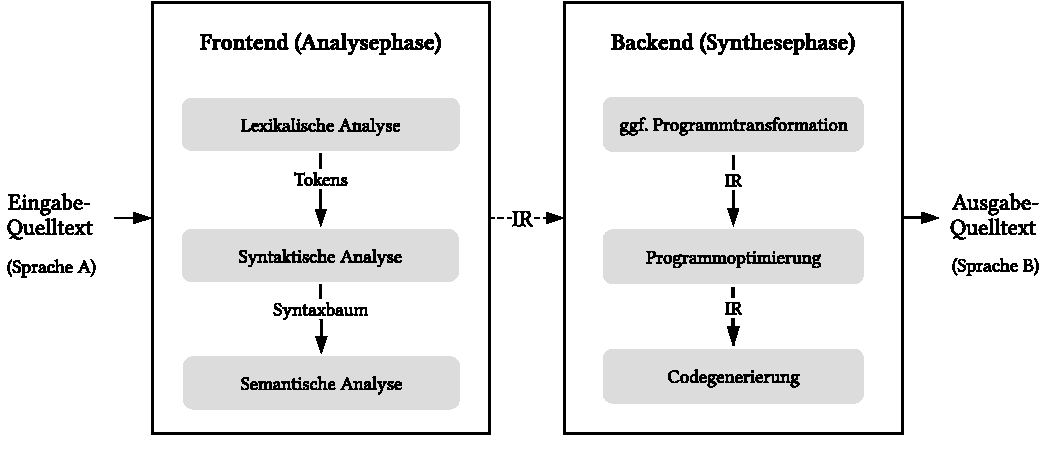
\includegraphics[width=\textwidth]{src/2_Grundlagen/fig/transpiler-architecture.pdf}
  \caption{Architektur eines typischen Transpilers nach~\autocite{EVGENIY:2016} und~\autocite[8]{TORCZON:2007}.}
	\label{fig:transpiler-architecture}
\end{figure}

Zunächst wird der Quelltext innerhalb der Analysephase durch den Lexer oder Tokenizer Zeichen für Zeichen eingelesen, um diesen in lexikalisch bedeutungsvolle Zeichenketten, sogenannte \emph{Lexeme} zu zerlegen~\autocite[43]{AHO:COMPILERS}. Daraufhin werden \emph{Tokens} gebildet, indem jedes dieser Wörter einer syntaktischen Klasse zugeordnet wird. Diese geben die Bedeutung eines Tokens an (zum Beispiel \code{3}~$\mapsto$~\code{INT(3)} oder \code{!=}~$\mapsto$~\code{NEQ})~\autocite[26]{TORCZON:2007}. Die Tokens entsprechen dabei den Terminalsymbolen der formalen Grammatik der Programmiersprache~\autocite[43]{AHO:COMPILERS}.

Im zweiten Schritt, der syntaktischen Analyse oder dem \emph{Parsen}, wird anschließend überprüft, ob die Tokenfolge eine Ableitung der kontextfreien Grammatik der Quellsprache darstellen, indem versucht wird einen entsprechenden \emph{konkreten} Syntaxbaum aufzubauen~\autocite{SCHOEPP:COMPILER}. Ein Syntax- oder Ableitungsbaum ist ein Graph, der die syntaktische Struktur eines Programms gemäß der zugehörigen Grammatik hierarchisch modelliert. Abbildung~\ref{fig:ast} zeigt exemplarisch den \emph{abstrakten} Syntaxbaum (AST) einer simplen JavaScript-Funktion. Ein abstrakter Syntaxbaum ist eine kompaktere Form des konkreten Baums und zeigt lediglich \enquote{wesentliche Teile}~\autocite[21]{WALDMANN:PPS} davon. Falls der Ableitungsbaum nicht erstellt werden kann, so liegt ein Syntaxfehler im Quelltext vor.

Danach prüft der Transpiler, ob ein gültiges Programm der Eingabesprache vorliegt, indem die statische Semantik analysiert wird~\autocite[8]{AHO:COMPILERS}. Hierunter fällt beispielsweise, dass Variablen in vielen Programmiersprachen vor deren Benutzung zunächst deklariert werden müssen. Um ein solches kontextuelles Programmverhalten zu untersuchen, können Attributgrammatiken verwendet werden~\autocite[161]{TORCZON:2007}. Während dieser Phase wird darüber hinaus die statische Typkorrektheit überprüft~\autocite{SCHOEPP:COMPILER}. Es ist hervorzuheben, dass nicht alle Transcompiler eine semantische Analyse durchführen.
Zuletzt wird durch das Frontend ein \emph{Zwischencode}\footnote{engl. \textit{intermediate representation} (IR).} des Programms erzeugt, der an das Backend übergeben wird. Ein Zwischencode ist im Allgemeinen eine von der Quellsprache und Zielarchitektur unabhängige Datenstruktur innerhalb von Compilern~\autocite[6]{TORCZON:2007}. Wie der nachfolgende Abschnitt zeigen wird, verwenden viele Transpiler im JavaScript-Umfeld den abstrakten Syntaxbaum als Zwischencode.

\begin{figure}[tb]
  {
    \begin{lstlisting}[numbers=none,aboveskip=0pt,belowskip=0pt]
    function square(x) {
      return x ** 2;
    }
    \end{lstlisting}
    \vspace{-0.5cm}
    \begin{center}
      \ttfamily
      \begin{forest}
        [FunctionDeclaration
          [Identifier, edge label={node[edge]{id}}
            [square, edge label={node[edge]{name}}]
          ]
          [Identifier{[]}, edge label={node[edge]{params}}
            [x, edge label={node[edge]{name}}]
          ]
          [BlockStatement, for tree = {s sep=1.3cm}, edge label={node[edge]{body}}
            [ReturnStatement, edge label={node[edge]{body}}
              [BinaryExpression, edge label={node[edge]{argument}}
                [Identifier, edge label={node[edge]{left}}
                  [x, tier=last, edge label={node[edge]{name}}]
                ]
                [**, tier=last, edge label={node[edge]{operator}}]
                [Literal, edge label={node[edge]{right}}
                  [2, tier=last, edge label={node[edge]{value}}]
                ]
              ]
            ]
          ]
        ]
      \end{forest}
    \end{center}
  }
  \caption{Abstrakter Syntaxbaum der obigen JavaScript-Funktion gemäß der Spezifikation \textit{ESTree}~\autocite{ESTREE_SPEC}.}
  \label{fig:ast}
\end{figure}

Der erste Schritt der Synthesephase besteht darin, das Programm sprachunabhängig zu optimieren, das heißt die Laufzeit oder den Speicherplatzbedarf auf Grundlage von Programmanalyse zu reduzieren~\autocite[405]{TORCZON:2007}. Hierbei können eine Vielzahl unterschiedlicher Transformationen angewandt werden. Möglich ist zum Beispiel die Entfernung nicht erreichbarer Programmstücke (\textit{dead code elimination}) oder die Inline-Ersetzung von Konstanten und Schleifen~\autocites{TORCZON:2007}{SCHOEPP:COMPILER}. Auch hier gilt es zu betonen, dass nicht alle Transcompiler eine derartige Optimierungsphase besitzen. Schließlich kann im letzten Schritt der endgültige Quelltext in der Zielsprache auf Basis des gegebenenfalls optimierten Zwischencodes erzeugt werden~\autocite[505]{AHO:COMPILERS}.

\subsection{Evaluation bestehender Transpiler für JavaScript}
\label{subsec:js-transpilers}

% \subsubsection{Anforderungen}

Im Umfeld von JavaScript sind im Lauf der Jahre eine Vielzahl von Parsern, Codegeneratoren und vollständigen Transcompiler entstanden, welche die Entwicklung weiterer Werkzeuge wie die des angestrebten Flow-Transpilers stark vereinfachen können. Im Folgenden sollen die relevantesten, aktuellen Ansätze bezüglich verschiedener Aspekte gegenüber gestellt werden, sodass daraufhin die Entscheidung getroffen werden kann, welches der Werkzeuge als Grundlage für die Umsetzung heran gezogen wird. Hierbei wird nur frei verfügbare, quelloffene Software betrachtet.

Die Auswahl hängt entscheidend von der Erfüllung mehrerer technischer Anforderungen ab, die auf Grundlage der gegebenen Rahmenbedingungen innerhalb des Unternehmens erarbeitet wurden. Diese werden in Kapitel~\ref{chap:analysis} ausführlich dargelegt. Die erste Vorgabe ist die vollumfängliche Unterstützung aktueller JavaScript-Syntax gemäß der ECMAScript-Spezifikation 2019~\autocite{ECMASCRIPT:2019} (ES10). Weiterhin muss die Verarbeitung von \emph{vorläufiger} Syntax möglich sein. Unter vorläufiger Syntax werden in dieser Arbeit Erweiterungen von JavaScript verstanden, die noch nicht endgültiger Bestandteil des Standards sind. Dieser wird stetig durch das \textit{Technical Committee 39} (TC39)~\autocite{TC39_COMMITTEE} weiterentwickelt. Vorgeschlagene Spracherweiterungen durchlaufen dabei einen mehrstufigen Standardisierungsprozess, der schließlich in die Aufnahme in die Spezifikation münden kann~\autocite{TC39_PROCESS}. Derartige Syntax einlesen zu können ist ebenfalls eine Anforderung, weil diese zum Teil bereits heute in den gegebenen Projekte von Spreadshirt eingesetzt werden\footnote{Dies setzt die Benutzung eines Transpilers wie Babel~\autocite{BABEL} voraus, der solche experimentelle Syntax vor der Auslieferung durch entsprechende Plugins in standardkonformes JavaScript transformiert.}. Damit die Übersetzung der Flow-Typen nach TypeScript möglich ist, muss ferner sowohl die Syntax von Flow, als auch von TypeScript vollständig unterstützt werden. Schließlich muss sogenannte JSX-Syntax~\autocite{SOFTWARE:JSX} (\textit{JavaScript XML}) eingelesen werden können, weil die zu migrierenden Projekte auch diese Notation verwenden.

% \subsubsection{Vergleich}

Tabelle~\ref{tab:transpilers} zeigt die Eigenschaften verschiedener Parser (\textit{Acorn}, \textit{Esprima}), Codegeneratoren (\textit{Astring}, \textit{Escodegen}) und Transpiler (\textit{Babel}, \textit{Recast}) für JavaScript. Jedes der Werkzeuge benutzt intern den abstrakten Syntaxbaum der Eingabe als Zwischencode. Weil abgesehen von Babel alle Alternativen die Spezifikation \textit{ESTree} als Format des abstrakten Syntaxbaums verwenden, können diese Parser und Codegeneratoren beliebig kombiniert werden, um einen Transcompiler zusammen zu setzen. Der ESTree-Standard wird von Mitgliedern verschiedener Projekte im Umfeld der statischen Analyse von JavaScript kontinuierlich weiterentwickelt und beschreibt den Aufbau abstrakter Syntaxbäume von ECMAScript-Programmen~\autocite{BABEL:PARSER,ESTREE_SPEC}.
Im Gegensatz zu den anderen betrachteten Optionen ist lediglich Babel und Recast in der Lage aktuelle und vorläufige JavaScript-Syntax, sowie Flow, TypeScript und JSX vollständig zu verarbeiten. In Recast wird dies jedoch nur durch die interne Verwendung Babels erzielt~\autocite{RECAST}. Recast ermöglicht die Verwendung einer Vielzahl unterschiedlicher Parser, um Quelltext-Transformationen umzusetzen. Da Babel im Vergleich zu Recast deutlich verbreiteter ist und aktiver entwickelt wird, kann Babel als die ausgereiftere Software betrachtet werden. Weiterhin kann Babel durch ein umfangreich dokumentiertes Plugin-Systems flexibel erweitert werden~\autocite{BABEL:HANDBOOK}. Aufgrund dieser Vorteile und Alleinstellungsmerkmale gegenüber den anderen Werkzeugen wird Babel als Grundlage für die Implementierung gewählt.

\begingroup
\setlength{\tabcolsep}{6pt} % reset to default
\begin{table}[tb]
  \footnotesize
  \begin{tabu} to \textwidth {@{}lllccccccrrX@{}}
    \midrule
    \libertineSB{Werkzeug} & \libertineSB{Typ} & \libertineSB{Format} & \libertineSB{Erw.} & \libertineSB{ES10} & \libertineSB{ES10+} & \libertineSB{Flow} & \libertineSB{TS} & \libertineSB{JSX} & \libertineSB{Aktivität} & \libertineSB{Sterne} \\
    \midrule
    Acorn     & P  &  ESTree  & \pie{2} & \pie{2} & \pie{1} & \pie{0} & \pie{0} & \pie{2} &   5 &  5.250 & {\autocite{ACORN}} \\ % 2012
    Astring   & G  &  ESTree  & \pie{2} & \pie{2} & \pie{1} & \pie{0} & \pie{0} & \pie{0} &  61 &    500 & {\autocite{ASTRING}} \\ % 2015
    Babel     & PG &  Babel   & \pie{2} & \pie{2} & \pie{2} & \pie{2} & \pie{2} & \pie{2} & 225 & 34.650 & {\autocite{BABEL}} \\ % 2014
    Escodegen & G  &  ESTree  & \pie{0} & \pie{0} & \pie{0} & \pie{0} & \pie{0} & \pie{0} &   2 &  1.900 & {\autocite{ESCODEGEN}} \\ % 2012
    Esprima   & P  &  ESTree  & \pie{0} & \pie{1} & \pie{0} & \pie{0} & \pie{0} & \pie{1} &  12 &  5.450 & {\autocite{ESPRIMA}} \\ % 2011
    Recast    & PG &  diverse & \pie{2} & \pie{2} & \pie{2} & \pie{2} & \pie{2} & \pie{2} &  43 &  2.700 & {\autocite{RECAST}} \\ % 2012
    \midrule
  \end{tabu}
  \caption*{
    \footnotesize
    \begin{minipage}[t]{.4\linewidth}
      {
        \renewcommand{\arraystretch}{1.1}
        \begin{tabular}{@{}ll@{}}
          P & Parser\\
          G & Codegenerator\\
          \pie{0} & keine Unterstützung\\
          \pie{1} & unvollständige Unterstützung\\
          \pie{2} & vollständige Unterstützung\\
        \end{tabular}
      }
    \end{minipage}
    \begin{minipage}[t]{.55\linewidth}
      {
        \renewcommand{\arraystretch}{1.1}
        \begin{tabular}{@{}ll@{}}
          Erw. & Erweiterbarkeit\\
          ES10 & ECMAScript 2019\\
          ES10+ & vorgeschlagene JavaScript-Erweiterungen\\
          TS & TypeScript\\
          Sterne & Anzahl der Sterne auf GitHub\\
        \end{tabular}
      }
    \end{minipage}

    \medbreak
    \begin{justify}
      Aktivität: Entspricht der Summe der Zahl von \emph{Merge Requests}, neuer bzw. geschlossener Fehlerberichte, veröffentlichter Git-Commits auf dem Hauptzweig und der Anzahl beteiligter Autoren innerhalb eines Monats auf der Plattform GitHub~\autocite{GITHUB} (Stand Oktober 2019).
    \end{justify}
  }
  \caption{Vergleich verschiedener Werkzeuge zur Transpilierung von JavaScript"=Quelltexten.}
  \label{tab:transpilers}
\end{table}
\endgroup


% https://babeljs.io/blog/2016/12/07/the-state-of-babel#the-future-parser-unity
% https://medium.com/@sebmck/2015-in-review-51ac7035e272#.jdoo279bl

% \subsubsection{Fazit}

\subsection{Babel}
\label{sec:babel}

\subsubsection{Funktionsweise}

Zur Erleichterung des Verständnisses der Ausführung der Umsetzung des Flow-Transpilers in Kapitel \ref{chap:implementation} soll zunächst die grundsätzliche Funktionsweise von Babel umrissen werden. Die Ausführung von Babel gliedert sich in folgende drei Phasen~\autocite{BABEL:HANDBOOK}. Diese sind in weiten Teilen analog zu dem beschriebenen Aufbau eines typischen Transcompilers.

\begin{enumerate}
  \item {\libertineSB{Parsen des Eingabecodes}}\\*
    Zunächst wird der ursprüngliche Quelltext in zwei Schritten eingelesen, um den abstrakten Syntaxbaum des Programms zu erzeugen: Als Erstes wird der Code während der lexikalischen Analyse mittels des Lexers in Tokens zerlegt. Anschließend werden diese in der syntaktischen Analyse zu einer Datenstruktur umgeformt, die den zugehörigen abstrakten Syntaxbaum repräsentiert. Jedem Knoten des Baums wird dabei einen eindeutiger Tokentyp zugewiesen, der die syntaktische Bedeutung widerspiegelt.
    \bigbreak
  \item {\libertineSB{Transformation des Programms}}\\*
    Während der zweiten Phase wird daraufhin die eigentliche Programmtransformation durchgeführt: Dabei wird der abstrakte Syntaxbaum durch das \emph{Besucher}"=Entwurfsmuster\footnote{Das Besucher-Entwurfsmustern (engl. \textit{visitor pattern}) gehört zu den 23 Entwurfsmustern, die im Standardwerk \citetitle{GAMMA:1994} der \enquote{\textit{Gang of Four}} (E. Gamma, R. Helm, R. Johnson und J. Vlissides) beschrieben werden~\autocite[306\psqq]{GAMMA:1994}.} rekursiv traversiert und die Knoten des Baums sukzessive modifiziert, gelöscht bzw. neu erstellte Elemente eingefügt. Das Entwurfsmuster beschreibt, wie ein Algorithmus auf einer komplexen Objektdatenstruktur, unabhängig von der konkreten Implementierung der zugrunde liegenden Klassen, ausgeführt werden kann~\autocite[634\psq]{FREEMAN:2004}. Im vorliegenden Fall ermöglicht die Anwendung die individuelle Adressierung einer bestimmten Untermenge der Knoten des Syntaxbaums, sodass dort die gewünschte Transformation des Programms durchgeführt werden kann.
    \bigbreak
  \item {\libertineSB{Generierung des Ausgabequelltexts}}\\*
    Schließlich kann der Ausgabecode generiert werden: Hierbei werden alle Knoten des abstrakten Syntaxbaums durch Anwendung einer Tiefensuche durchlaufen und eine Zeichenkette aufgebaut, die den endgültigen, modifizierten Quelltext darstellt.
\end{enumerate}

\subsubsection{Babel-Plugins}
\label{subsec:babel-plugins}

Da die entscheidende Phase der Transpilierung, die Programmtransformation, bei Babel durch Plugins erzielt wird, sollen diese genauer betrachtet werden. Plugins sind die elementaren Bausteine, die eine flexible Erweiterung von Babel ermöglichen. Selbst der Kern des Transcompilers ist aus einer Vielzahl von Standard-Plugins zusammen gesetzt, die in ihrer Gesamtheit die Funktionalität des Systems abbilden~\autocite{BABEL}. Dies verdeutlicht die tiefgreifende Modularität der Architektur von Babel. Jedes Plugin ist eine JavaScript"=Funktion, welche gemäß der vorgegebenen Schnittstelle ein Objekt mit verschiedenen Attributen zurückliefern muss. Mindestens anzugeben ist dabei lediglich die Abbildung der gewünschten Knotentypen des abstrakten Syntaxbaums auf Besucherfunktionen~\autocite{BABEL:HANDBOOK}. Deren Implementierung setzt die angestrebte Quelltext"=Transformation um. Es ist in der Praxis gängig mehrere Plugins einzusetzen, sodass ein Knoten während der Verarbeitung durch Babel mehrere, unabhängige Transformationen durchlaufen kann. Hierdurch kann die erwünschte Transpilierung von JavaScript-Quelltexten flexibel durch Kombination vieler, kleiner Bausteine realisiert werden. Auch möglich ist die Angabe einer hierarchischen Abhängigkeitsstruktur, sodass dass die Verwendung eines Plugins zur impliziten Aktivierung weiterer Plugins führt.

\begin{lstlisting}[
  float,
  floatplacement=H,
  label={code:babel-plugin-definition},
  caption={[Minimalbeispiel eines Babel-Plugins]Minimalbeispiel eines Babel-Plugins: Die Namen aller Bezeichner (\code{Identifier}) werden in Großbuchstaben umgewandelt.}
]
// var foo => var FOO
module.exports = function() {
  return {
    visitor: {
      Identifier(path) {
        path.node.name = path.node.name.toUpperCase();
      }
    }
  };
};
\end{lstlisting}

Der konkrete Aufbau von Babel-Plugins soll durch ein Minimalbeispiel gezeigt werden. Quelltext~\ref{code:babel-plugin-definition} zeigt den Code eines simplen aber vollständigen Plugins, welches lediglich den Namen aller Bezeichner (\code{Identifier}) eines JavaScript-Programms in Großbuchstaben setzt. Hierfür wird eine gleichnamige Besucherfunktion für den Knotentyp \code{Identifier} definiert (Zeile 5). Diese erhält den \emph{Pfad} der so adressierten Identifier-Knoten als Argument und kann diesen wie gewünscht transformieren. Der Pfad eines AST-Knotens ist ein Objekt, das die Beziehung des Knotens zu seinen Elternelementen modelliert und diesen um Metainformationen anreichert~\autocite{BABEL:HANDBOOK}. Es enthält eine Vielzahl von Methoden mittels derer der Pfad und der Syntaxbaum manipuliert werden kann.
Alle Knotentypen des abstrakten Syntaxbaums werden einerseits in der Spezifikation des Parsers von Babel~\autocite{BABEL:PARSER_SPEC,BABEL:PARSER}, andererseits in der Dokumentation der Bibliothek \code{@babel/types}~\autocite{BABEL:TYPES} beschrieben.
Der Aufbau des von Babel eingesetzten abstrakten Syntaxbaums liegt in einem eigenen Format vor, das ursprünglich auf dem ESTree-Standard~\autocite{ESTREE_SPEC} basiert. Grund für die Abspaltung Babels von der ESTree-Spezifikation seit der sechsten Version ist, dass das Projekt auch vorläufige JavaScript-Erweiterungen unterstützen möchte~\autocite{BABEL:STATE_OF_BABEL}.

Im weitere Verlauf wird das Hauptaugenmerk der Untersuchung auf die zweite Phase der Transpilierung durch Babel gelegt, da hier die vorliegende Problemstellung, die Transformation der Flow-Typannotationen nach TypeScript, umgesetzt wird. Das Parsen des Eingabquelltexts und das Generieren der Ausgabe kann durch Verwendung der gegebenen Bibliotheksfunktionen von Babel simpel realisiert werden und bedarf keiner tiefgründigen Betrachtung.
